In this section, the Server Layer is described in terms of the hardware and software design. 

\subsection{Layer Operating System}
The operating system for the server is current project is Windows Server however, any server based operating system is acceptable so long as it can run PHP and MySQL.

\subsection{Subsystem 1}
Script Subsystem is a portion of every .php file on the website. This data flows from HTML pages into the PHP scripts which use the information in SQL statements to retrieve or send data to the database. Then, PHP generates code for HTML output.

\begin{figure}[h!]
	\centering
 	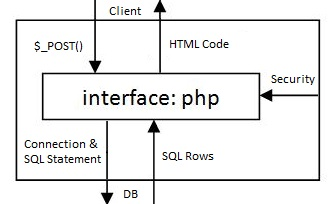
\includegraphics[width=0.60\textwidth]{images/PHPScriptSubsystem}
 \caption{Dataflow of the PHP Scripting Subsystem}
\end{figure}

\subsubsection{Subsystem Operating System}
This subsystem depends only on the layer Operating System requirements.

\subsubsection{Subsystem Programming Languages}
This subsystem is based purely on PHP code. This subsystem often generates HTML5 based code for client side use and SQL statements to be sent to the database.

\subsection{Subsystem 2}
The website's storage system. Internet host stores code, script and image files to be used on the website. 

\begin{figure}[h!]
	\centering
 	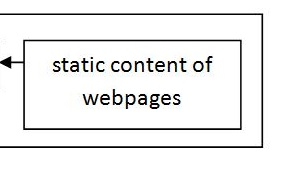
\includegraphics[width=0.40\textwidth]{images/FileStorageSubsystem}
 \caption{Files are sent out when needed}
\end{figure}

\subsubsection{Subsystem Operating System}
This subsystem depends only on the layer Operating System requirements.

\subsubsection{Subsystem Data Processing}
Data files are accessed and sent out after successful Client-Server handshakes.